\documentclass[10pt,twocolumn,letterpaper]{article} 

\usepackage{avss}
\usepackage{times}
\usepackage{epsfig}
\usepackage{graphicx}
\usepackage{amsmath}
\usepackage{amssymb}


\usepackage[colorlinks,
linkcolor=red,
anchorcolor=blue,
citecolor=green
]{hyperref}


% Include other packages here, before hyperref.

% If you comment hyperref and then uncomment it, you should delete 
% egpaper.aux before re-running latex.  (Or just hit 'q' on the first latex
% run, let it finish, and you should be clear).
%\usepackage[pagebackref=true,breaklinks=true,letterpaper=true,colorlinks,bookmarks=false]{hyperref}


%\avssfinalcopy % *** Uncomment this line for the final submission

\def\avssPaperID{21} % *** Enter the AVSS Paper ID here
\def\httilde{\mbox{\tt\raisebox{-.5ex}{\symbol{126}}}}

% Pages are numbered in submission mode, and unnumbered in camera-ready
\ifavssfinal\pagestyle{empty}\fi
\begin{document}

%%%%%%%%% TITLE
\title{Efficient 3D Convolutional Neural Networks for Violence Detection}

\author{First Author\\
Institution1\\
Institution1 address\\
{\tt\small firstauthor@i1.org}
% For a paper whose authors are all at the same institution, 
% omit the following lines up until the closing ``}''.
% Additional authors and addresses can be added with ``\and'', 
% just like the second author.
% To save space, use either the email address or home page, not both
\and
Second Author\\
Institution2\\
First line of institution2 address\\
{\tt\small secondauthor@i1.org}
}

\maketitle
% \thispagestyle{empty}

%%%%%%%%% ABSTRACT
\begin{abstract}
Automatically analyzing violent content in surveillance videos is of profound significance on many applications, ranging from video content filtration to public security protection. Recognition accuracy and computational efficiency are two key factors to perform this task. In this paper, we propose a deep learning model based on 3D convolutional neural networks with improved internal architecture, which is more capable of capturing spatiotemporal features and requires relatively fewer parameters. The proposed model is validated on three standard datasets in terms of classification accuracy. Meanwhile, supplementary experiment is carried out to evaluate its effectiveness and efficiency. The final results demonstrate the advantages of our model over the state-of-the-art approaches in both recognition accuracy and computational efficiency.
\end{abstract}

%%%%%%%%% BODY TEXT
\section{Introduction}
\label{sec:1}

Nowadays, violence and terrorist attack have become primary threats to world security and stability.
Thanks to the development of digital media technologies, violent scenes can be recorded by surveillance cameras.
However, with a large number of video materials produced every moment, it is unrealistic to manually guard these videos and capture every violent scene in real time.
Consequently, it is of profound significance to develop an efficient system which can automatically monitor and detect violence in surveillance videos.
In current tasks, violence is considered as aggressive behaviors of human, rather than fire, shots, explosion or blood.
Based on the above conception, there are three standard benchmark datasets constructed for performance evaluation.
We follow the meaning of violence in this work to keep consistent with related researches.

In recent years, computer vision has been continuing to evolve with the improvement of computing power and the availability of large-scale datasets.
Deep learning, a critical technology in computer vision, has achieved remarkable milestones in many fields, such as image classification and object detection.
It has also been introduced to address the problem of violence detection in videos.
Compared to approaches based on hand-crafted features, deep learning methods yield tremendous improvements in robustness and recognition accuracy.
However, there may be trade-offs and hard choices when considering both computational efficiency and recognition accuracy.
Consequently, developing an effective and efficient deep learning model is very crucial in practical applications.

In view of the circumstances above, we leverage the latest research findings in computer vision and develop a deep learning model for violence detection. Our major contributions are summarized as follows:
\begin{itemize}
	\item We propose a deep learning model based on 3D CNNs with improved internal architecture for violence detection tasks.
	\item We demonstrate that properly selected internal architectures can improve the ability of representing abstract spatiotemporal information and reducing the number of parameters.
	\item We experimentally validate our model on three standard benchmark datasets and conduct supplementary experiment to evaluate the effectiveness and efficiency of our model.
\end{itemize}

The rest of the paper is organized as follows: Section \ref{sec:2} introduces the related works and approaches for violence detection. Section \ref{sec:3} explains the details of the proposed method, followed by experiment and analysis in Section \ref{sec:4}. Finally, Section \ref{sec:5} concludes the work in this paper.

%------------------------------------------------------------------------

\section{Related Work}
\label{sec:2}

In earlier studies, violence detection approaches generally depend on the recognition of specific visual cues like flame and blood together with audio content such as gunshot or breaking sound \cite{nam1998audio, cheng2003semantic, zajdel2007cassandra}.
However, in most cases, surveillance cameras do not contain audio devices, which brings great difficulties to audio based approaches. 
Therefore, methods based on videos become the mainstream of this field. 
Video based approaches, typically can be divided into two categories according to their feature extraction methods: 
traditional hand-crafted feature based approaches and deep learning approaches.

Hand-crafted approaches usually extract frame-level features designed by human, then aggregate them using encoding strategies, and finally apply machine learning classifiers for the final decision.
Among these approaches, STIP \cite{STIPs}, MoSIFT \cite{MoSIFT} and iDT \cite{iDTs} are widely used features for violence detection such as \cite{vio_sift, hockey, mosift_sc}.
There are also several descriptors specifically designed for representation of violence information. 
Hassner et al. \cite{vif} introduced VIolent Flows (ViF) feature by estimating magnitude of optical flow over time.
Later, Gao et al. \cite{ovif} improved this work and proposed Oriented VIolent Flows (OViF) feature by additionally calculating statistical motion orientations.
Deniz et al. \cite{fast} applied Radon Transform on the power spectrum of consecutive frames to estimate extreme acceleration patterns in fights.
Bilinski et al. \cite{bilinski2016human} developed an extension of Improved Fisher Vectors for videos to represent local features and their spatio-temporal positions.
Zhang et al. \cite{MoIWLD} proposed a modified motion Weber local descriptor (MoIWLD) as the new feature descriptor.
Deb et al. \cite{vlad} introduced Outlier-Resistant VLAD (OR-VLAD) to improve the performance for feature encoding.

Deep learning approaches, differently from traditional methods, use trainable deep neural networks as feature extractor, and usually build an end-to-end model including feature extraction, encoding, and classification. 
Simonyan et al. \cite{two-stream} firstly proposed two-stream networks for human action recognition by adding extra temporal network to capture motion information in optical flows.
Dong et al. \cite{dong2016multi} extended this model to multi-stream, adding another acceleration stream for capturing intense motion in violence. Also, they employed LSTM \cite{lstm} network to model long-term information.  
Zhou et al. \cite{zhou2017violent} applied temporal segment networks (TSN) \cite{tsn} and proposed FightNet model. This model takes raw frames, optical flow, and acceleration field as input and SoftMax is used for final fusion.
Serrano et al. \cite{serrano2018fight} employed Hough Forests to build representative image for each video sequence, followed by a 2D ConvNets for the final decision.

These approaches leverage the hand-crafted features by combining them with deep learning technologies.
However, drawbacks are that they are not end-to-end trainable and are more dependent on the effectiveness of hand-crafted features.
Besides, it may be inefficient to add additional computation steps. 

Several end-to-end trainable models have been proposed to solve these problems.
Ding et al. \cite{3dcnn_ding} proposed a 3D ConvNets for violence detection without using any hand-crafted feature or prior knowledge. 
Sudhakaran et al. \cite{convlstm_sudh} applied 2D ConvNets to extract spatial feature maps, then followed by ConvLSTM \cite{convlstm} to encode spatiotemporal information.
This work was subsequently improved by Hanson et al. \cite{bi_convlstm} by building Bidirectional ConvLSTM (Bi-ConvLSTM) architecture as spatiotemporal encoder.

Recently, deep learning methods based on 3D CNNs have achieved tremendous success in the field of action recognition, owing to the availability of large scale datasets and the improvements of technologies. 
Tran et al. \cite{3dcnn_1} proposed C3D discriptor and raised four properties for effective video descriptors: generic, compact, efficient and simple. 
Carreira et al. \cite{kinetics} built a large scale dataset called Kinetics for human action recognition, which plays a significant role similar to that ImageNet \cite{imagenet} plays in image recognition. 
Soon after, Hara et al. \cite{3dcnn_2} conducted a series of experiments and demonstrated that 3D CNNs pre-trained on Kinetics dataset could retrace the triumph of 2D CNNs and ImageNet.
Tran et al. \cite{r2+1d} explored several varieties of 3D CNN architectures and designed a new spatiotemporal convolutional block called R(2+1)D for action recognition.
Also, they comprehensively studied several good practices for applying 3D CNNs to specific tasks.

By taking full advantage of recent research findings, we develop an efficient and effective 3D CNN model with specifically designed architecture for violence detection tasks.


%------------------------------------------------------------------------- 

% figures

\begin{figure*}
\begin{center}
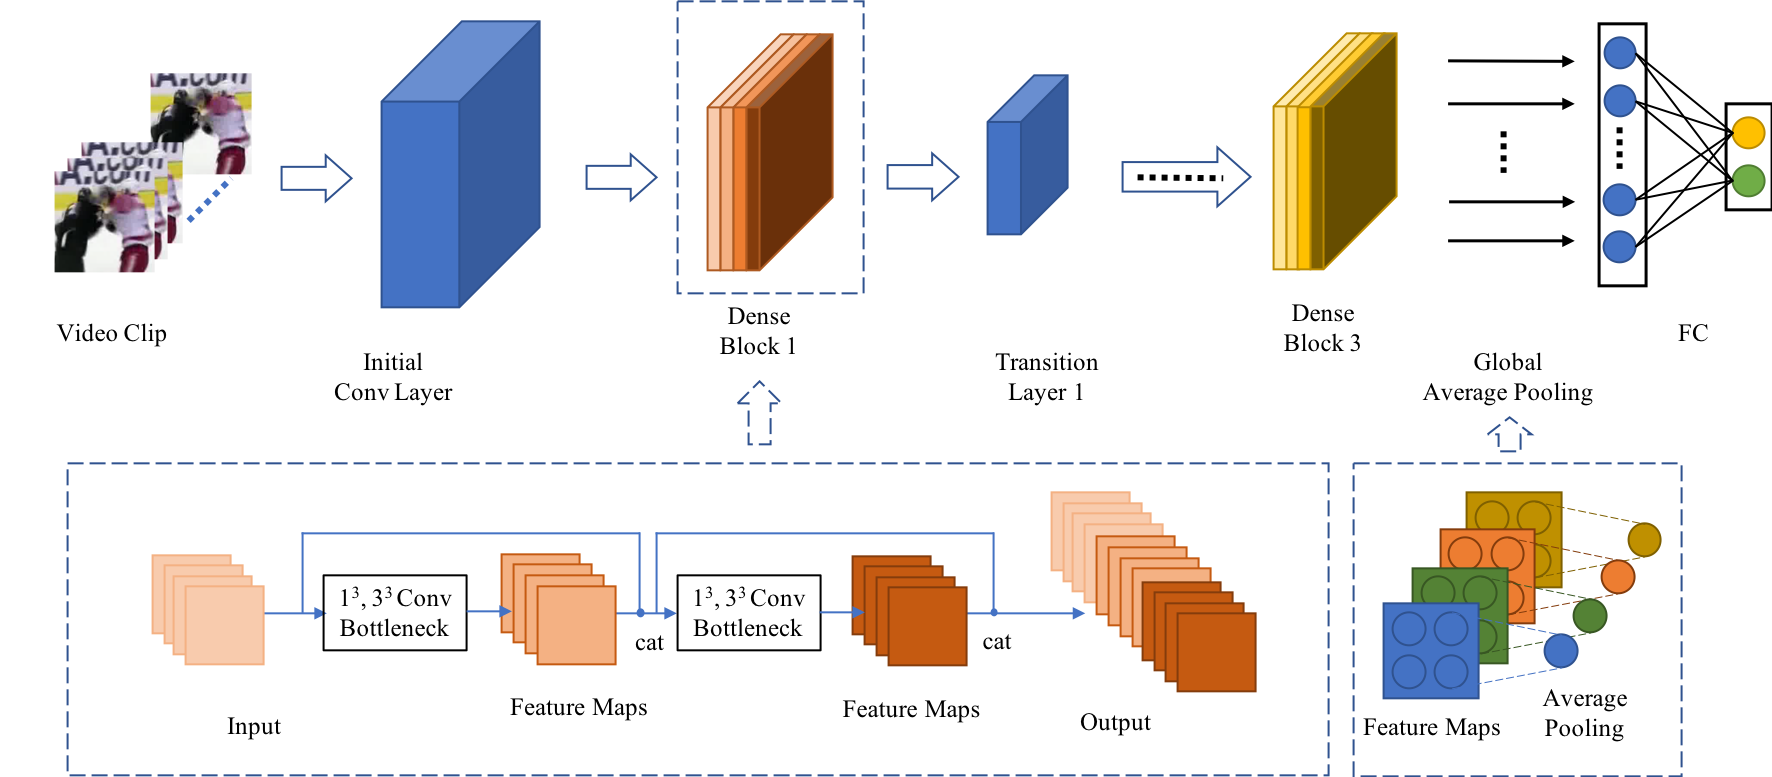
\includegraphics[scale=0.52]{fig/fig1.png}
\end{center}
\caption{Block diagram of the proposed model. The model is composed of one initial convolution layer, three dense blocks, two transition layers, and one fully connected layer (Dense Block 2 and Transition Layer 2 are omitted due to limitation of space). Each dense block contains several dense layers. The fully-connected layer are joined with output feature maps using global averaging pooling strategy.}
\label{fig:model}
\end{figure*}
	
	
%------------------------------------------------------------------------- 

\section{Proposed Method}
\label{sec:3}

The purpose of the proposed method is to design an end-to-end trainable deep learning model for detecting and recognizing fight clips in videos. 
For a model able to identify violent scenes, it should be capable of capturing anomaly or intense motions pattern of human bodies. 
Recognition accuracy and computational efficiency are two important indicators.
Consequently, developing effective and efficient spatiotemporal modules is of great importance in this task.
In view of the facts above, we leverage the findings in \cite{3dcnn_1, 3dcnn_2, r2+1d} and refer to the successful architecture of DenseNet \cite{densenet}, then finally develop a deep learning model based on 3D convolutional networks.

\subsection{Rethinking 3D Convolutional Networks}

For video understanding tasks, the most critical issue is how to extract appropriate features that are representative of the spatiotemporal information.
Compared to those architectures that separately encode spatial and temporal information, 3D CNNs can simultaneously capture spatiotemporal features as its convolution kernel extended to three dimensions. 
It implies that there is no need to apply extra LSTM or other RNN architectures exclusively designed for encoding temporal information. 
Also, raw pixels can be input directly without complex preprocessing or extra calculation, which is much more computationally efficient than other deep learning model using optical flow, trajectories, and so forth.

However, the number of parameters may  exponentially increase as 3D convolution filters cube the kernel size, which may bring two main problems: 
Firstly, more parameters require higher FLOPs, which is computational inefficient; 
Secondly, redundant parameters may result in model overfitting and decreased generalization ability, especially in small scale datasets. 
To address these problems and promote 3D CNNs to give scope to its representation potentials, we have adopted several strategies.

The most direct way is to reduce the kernel size of convolution filters. 
For instance, two serialized 3$\times$3$\times$3 kernels have nearly the same representation ability of one 5$\times$5$\times$5 kernel, while the number of parameters is only half. 
Also, findings in \cite{3dcnn_1, 3dcnn_2, r2+1d} suggest that 3$\times$3$\times$3 kernel size is the best option for 3D CNNs.

Encouraging feature reusing is also a good practice in designing networks. 
In the model training phase, it helps to facilitate the backpropagation of information flow, which conduces to avoid overfitting and improve generalization. 
DenseNet \cite{densenet} gives serials of inspirations on developing compact but effective network architectures.

\subsection{Network Architecture}

An overview of the proposed model is illustrated in Figure \ref{fig:model}, including three dense blocks and two transition layers. 
All the kernel sizes of convolution filters and pooling layers are three-dimensional. 
The network takes video clips as inputs, from which the initial convolution layer produces primary 64 feature maps. 
Then these feature maps are handled in the following first dense block. 
Dense block composes of several densely connected layers, namely dense layers.
The $l^{th}$ dense layer receives all the feature maps produced by its preceding layers, $y_0$, $y_1$, $\cdots$, $y_{l-1}$, as inputs:
\begin{equation}
\label{eq:densenet}
y_l = H_l\left([y_0, y_1, \cdots, y_{l-1}]\right)
\end{equation}
where $H_l(*)$ is the state transition function of the $l^{th}$ layer, and $[*]$ denotes concatenating operation.
Each dense layer produces $k$ new feature maps, where $k$ is a hyper-parameter called growth rate. 
For a dense block containing $L$ layers, it produces $k \times L$ new feature maps.
Diagram in the left dashed box of Figure \ref{fig:model} illustrates a simplified mechanism in dense block, where the number of dense layers is 2 and the growth rate $k$ is 4.
It outputs 12 feature maps, 8 of which are newly produced by its dense layers.

At the end of this model, we adopt global average pooling strategy proposed in \cite{NinN} to bridge the convolutional networks with fully connected layer for classification.
As is illustrated in the right dashed box of Figure \ref{fig:model}, the final output feature maps ($T \times H \times W$ tensors) are separately pooled into scalars.
It is conducive to avoid overfitting and can improve the generalization ability of the model. 
Meanwhile, it is more parameter saving compared to direct connection, implying a better computational efficiency.

Violent or aggressive behaviors contain not only simple movement patterns but also abstract high-order features like acceleration, duration, and body interaction.  
By feature reusing, the collective knowledge in every stage of the model is preserved and utilized by the final classifier for the final judgment, or rather a fusion based on the diversified and composed features, which can achieve more robust and generalized model. 

%------------------------------------------------------------------------- 

\begin{figure}[t]
\begin{center}
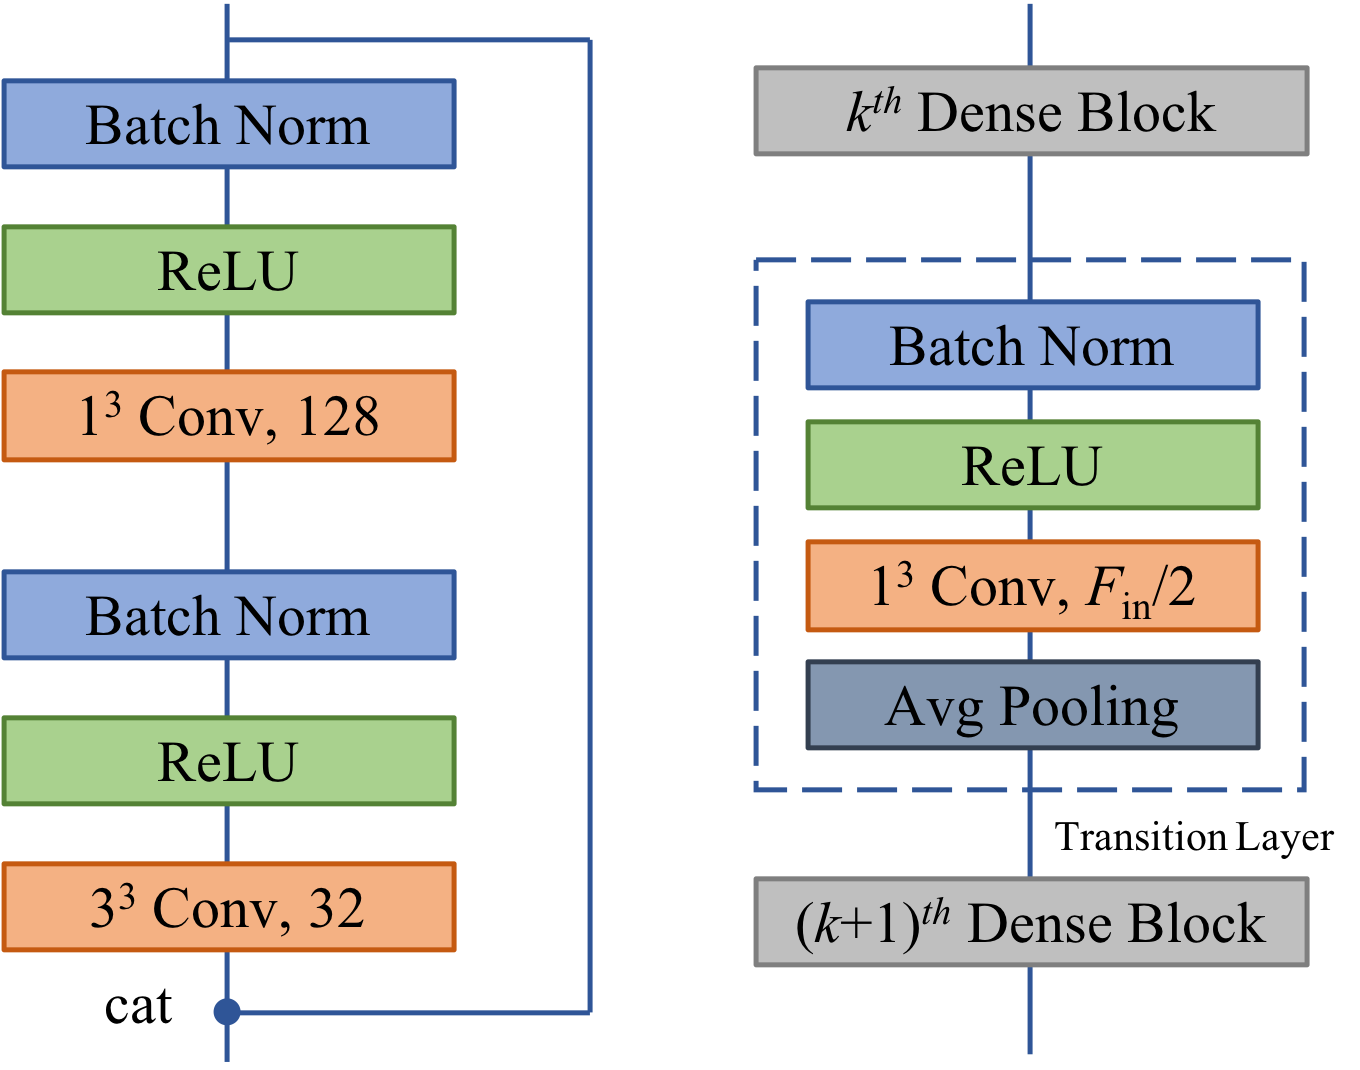
\includegraphics[scale=0.30]{fig/fig2.png}
\end{center}
\caption{Block diagram of bottleneck and transition layer. The block [$x^3$ Conv, $F$] denotes a convolution filter that have the kernel size of $x \times x \times x$ and produces $F$ feature maps.}
\label{fig:bottleneck}
\end{figure}

\begin{table}[b]
\begin{center}
\caption{Network architecture of the proposed model.}
\label{table:arch}
\begin{tabular}{lcr}
\hline
\textbf{Module Name} & \textbf{Architecture} & \textbf{Output Shape} \\
\hline\hline
Input Clip & - & [3,16,112,112] \\
Initial Conv & $7^3$ Conv, (1,2,2) & [64,16,56,56] \\
Pooling & $3^3$ Max & [64,8,28,28] \\
DenseBlock 1 & $(1^3, 3^3) \times 6$ & [256,8,28,28] \\
TransitionLayer 1 & $1^3$ Conv, $3^3$ Avg & [128,4,14,14]\\
DenseBlock 2 & $(1^3, 3^3) \times 12$ & [512,4,14,14] \\
TransitionLayer 2 & $1^3$ Conv, $3^3$ Avg & [256,2,7,7] \\
DenseBlock 3 & $(1^3, 3^3) \times 24$ & [1024,2,7,7]\\
GlobalAvgPooling & $2 \times 7 \times 7$ Avg & [1024,1,1,1]\\
Classification & FC Layer & [2, -, -, -] \\
\hline
\end{tabular}
\end{center}
\footnotesize
For $3^3$ convolution and pooling, the default stride is (2,2,2). The $(1^3, 3^3)$ denotes the bottleneck architecture in Figure \ref{fig:bottleneck}.
\end{table}

%------------------------------------------------------------------------- 

\subsection{Internal Details}

Dense layer should be elaborately designed since it is the basic unit for feature learning. 
Here, \emph{Bottleneck} architecture with pre-activation is adopted in every dense layer. 
The left diagram in Figure \ref{fig:bottleneck} represent the bottleneck architecture, whose growth rate is 32 and bottleneck size is 4.
The $1 \times 1 \times 1$ convolution layer produces $32 \times 4$ intermediate feature maps, followed by $3 \times 3 \times 3$ convolution layer that produces 32 (growth rate) output feature maps.
Typically, dense layer on the later place has more inputs as it receives all the feature maps from its preceding layers. 
Consequently, using bottleneck helps to compact feature maps, thus improves computational efficiency.
Meantime, the expansion inside bottleneck promotes infomation interaction between different channels, which is favorable for learning complex features.

Transition layer is placed between any two dense blocks, as is illustrated in the right diagram of Figure \ref{fig:bottleneck}.
The objective of placing transition layer is to downsample feature maps and match the number of output and input feature maps between adjacent blocks.
Here we set the number of output feature maps equal to half of the input, as $F = F_{in}/2$.
In addition to reducing the complexity and tuning the nonlinearity of the model, the transition layer can also help to promote interaction between channels, which enhances the feature learning ability and improves the robustness of our model.

Table \ref{table:arch} lists the details of the proposed model.
In the column of output shape, $[F, T, H, W]$ denotes the shape of tensors (feature maps) produced by the corresponding module.
Note that dense blocks are slightly different from the simplified illustration in Figure \ref{fig:model} as they use the bottleneck in Figure \ref{fig:bottleneck}. 

%------------------------------------------------------------------------ 




%------------------------------------------------------------------------ 

\begin{table*}
\begin{center}
\caption{Comparison of classification accuracy on three standard datasets.}
\label{table:result}
\begin{tabular}{lccc}
\hline
\textbf{Method} & \textbf{Hockey Fights Dataset} & \textbf{Movies Dataset} & \textbf{VIolent Flows Dataset} \\
\hline\hline
ViF + OViF \cite{ovif} & 87.5$\pm$1.7\% & - & 88$\pm$2.45\% \\
Radon Transform \cite{fast} & 90.1$\pm$0\% & 98.9$\pm$0.22\% & - \\
STIFV \cite{bilinski2016human} & 93.4\% & 99\% & 96.4\% \\
MoIWLD \cite{MoIWLD} & 96.8$\pm$1.04\% & - & 93.19$\pm$0.12\% \\
OR-VLAD \cite{vlad} & 98.2$\pm$0.76\% & \textbf{100$\pm$0\%} & 93.09$\pm$1.14\% \\
\hline
Three streams + LSTM \cite{dong2016multi} & 93.9\% & - & - \\
FightNet \cite{zhou2017violent} & 97.0\% & 100\% & - \\
Hough Forests + CNN \cite{serrano2018fight} & 94.6$\pm$0.6\% & 99$\pm$0.5\% & - \\
ConvLSTM \cite{convlstm_sudh} & 97.1$\pm$0.55\% & \textbf{100$\pm$0\%} & 94.57$\pm$2.34\% \\
Bi-ConvLSTM \cite{bi_convlstm} & 98.1$\pm$0.58\% & \textbf{100$\pm$0\%} & 93.87$\pm$2.58\% \\
\textbf{Proposed} & \textbf{98.3$\pm$0.81\%} & \textbf{100$\pm$0\%} & \textbf{97.17$\pm$0.95\%} \\
\hline
\end{tabular}
\end{center}
\end{table*}

%------------------------------------------------------------------------ 

\section{Experiments and Analyses}
\label{sec:4}

Experiment has been conducted to validate the performance of the proposed model on three standard benchmark datasets.
Meanwhile, in the supplementary experiment, effectiveness and efficiency are also evaluated.

\subsection{Dataset}

In violence detection tasks, there are three public standard benchmark datasets: \\
\textbf{Hockey Fights Dataset} \cite{hockey} contains 1000 videos collected from hockey games.
Each video consists of 50 frames with 720$\times$576 pixels. Nearlly all of the videos have the same background and human activities including fights and normal gamings. \\
\textbf{Movies Dataset} \cite{hockey} has 200 untrimmed video clips obtained from action movies with different resolutions. Different from Hockey, videos in Movies dataset vary in contents.\\
\textbf{VIolent-Flows Dataset} \cite{vif} consists of 246 videos of crowd behavior with frames resized to 320$\times$240 pixels.
Different perspectives, noisy background and dense crowd make this dataset relatively challenging for feature learning.

All of these three datasets contain balanced fight and non-fight samples. 
However, as designed for hand-crafted methods, these datasets are relatively small in scale, which may not be capable of training deep neural networks.
To cope with this problem, the ConvLSTM method \cite{convlstm_sudh} uses AlexNet model pre-trained on ImageNet.
Similarly, we consult the conclusion in \cite{3dcnn_2} and employ part of the parameters in their model which is pre-trained on Kinetics dataset \cite{kinetics}.
These parameters are imported to initialize the first convolution layer in our model.

The three datasets are also mixed up as Mix dataset.
In Mix dataset, positive and negative samples are randomly drawn from original datasets separately in the same proportion.
Mix dataset can be used to evaluate overall performance for deep learning models of their modeling capability and generalization ability in violence detection task.

\subsection{Experiment Setup}

The proposed model is implemented using PyTorch \cite{pytorch} platform. 
When comparing inference speed, other deep models for comparision are also implemented with PyTorch to guarantee comparability and consistency.

The inputs of network are prepared as tensors with shape $N \times C \times T \times H \times W$, where $N$ is the batch size, $C$ is the number of channels (3 for RGB videos), $T$ is the duration of clips and $H \times W$ is the frame resolution. 
In the experiment, each video is extracted with 16 adjacent frames and then cropped and resized into 112$\times$112 pixels.

In the training phase, data augmentation is employed to enlarge training set and reduce overfitting, including random horizontal flipping, spatially random scale cropping and temporally random slicing. 
The learning rate and batch size are $10^{-3}$ and $32$ for Hockey and $10^{-4}$ and $16$ for Movie and ViF, considering the scales of dataset.
We apply mini-batch stochastic gradient descent (SGD) with momentum 0.5 and weight decay $10^{-3}$ for model optimization.  
Cross entropy function defined in \ref{eq:crossentropy} is used for loss calculation. 
\begin{equation}
\label{eq:crossentropy}
\operatorname{loss}(x, \text{label}) = -\log \left(\frac{\exp (x[\text{label}])}{\sum_{j} \exp (x[j])}\right)
\end{equation}

In the evaluation phase, videos in test set are spatially cropped around center position and temporally sliced to use centre adjacent frames.

For supplementary experiment on Mix dataset, we split it into training set and validation set with 9:1, as there are totally 1,446 videos. 
The proposed model is still trained by SGD algorithm with momentum, while ConvLSTM \cite{convlstm_sudh} model is optimized using RMSprop algorithm.
The batch size is set to 32 and learning rate is set to $10^{-3}$.

\subsection{Results and Analyses}

In the experiment, we adopt five-fold cross validation to evaluate the recognition performance of the proposed method to keep consistent with the previous methods.
Table \ref{table:result} gives the classification accuracy of the state-of-the-art methods on three standard datasets, with deep learning methods listed in the lower half of the table and hand-crafted methods in the upper half.
From this table, it can be seen that deep learning methods, generally perform better than hand-crafted methods.
Among them, the proposed method achieves the best performance on all of these three datasets.

As explained in Section \ref{sec:1}, violence is considered as aggressive behaviors of human. 
Consequently, it may be obscure to distinguish fights from ohter human body movements like sports and celebrations.
Taking Hockey Fights dataset for example, normal games can also contain body collision or powerful strokes, which can be confusing and have a real possibility to be mistaken as violence.
Nevertheless, the proposed model obtains the highest accuracy, implying that it is capable capturing spatiotemporal motion cues and high order localized region information. 
In the case of Movies dataset, since it has easily identifiable positive and negative samples, every model performs well.
As for VIolent-Flows dataset, dense crowd and noisy background make it challengeable to capture violent cues. 
Also, multi-scale and multi-viewpoint may be  another two factors that effect model performance.
Nevertheless, owing to the design of feature reusing and the global field of final decision, the proposed method forms a multi-attention mechanism for discovering violent position in videos.

%------------------------------------------------------------------------ 

\begin{table}
\begin{center}
\caption{Experiment results on Mix dataset.}
\label{table:mix}
\begin{tabular}{lccc}
\hline
\textbf{Model} & \textbf{Accuracy} & \textbf{CE Loss} & \textbf{\# Params} \\
\hline\hline
C3D \cite{3dcnn_1} & 92.47\% & 0.4019 & 78.0M \\
ConvLSTM \cite{convlstm_sudh} & 96.58\% & 0.1355 & 9.6M \\
\textbf{Proposed} & \textbf{99.32\%} & \textbf{0.0326} & \textbf{7.4M} \\
\hline
\end{tabular}
\end{center}
\end{table}

\begin{figure}[t]
\begin{center}
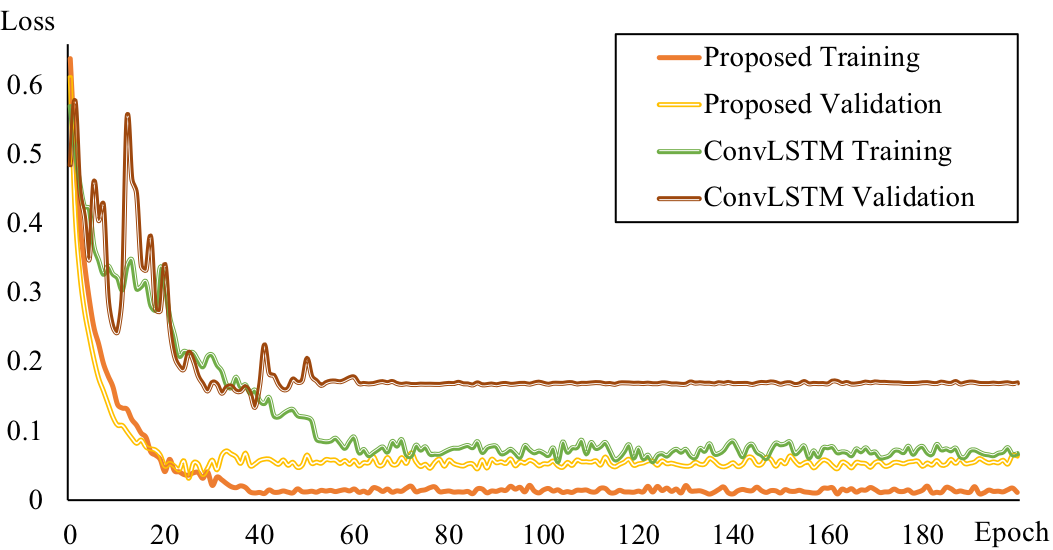
\includegraphics[scale=0.46]{fig/fig3.png}
\end{center}
\caption{Training and validation losses of the proposed model and ConvLSTM \cite{convlstm_sudh} on Mix dataset.}
\label{fig:mix}
\end{figure}

%------------------------------------------------------------------------ 

Supplementary experiment on Mix dataset is carried out to evaluate comprehensive performance of deep learning model.
Due to the limited conditions, we only evaluate our model with two classic methods, C3D \cite{3dcnn_1} and ConvLSTM \cite{convlstm_sudh}. 
As is given in Table \ref{table:mix}, the proposed model has better classification with relatively fewer parameters.
Its cross entropy loss on validation set is an order of magnitude lower than those of two other models.
Also, Figure \ref{fig:mix} illustrates the details of training and validation epochs. 
Compared to ConvLSTM, the proposed model is faster in convergence and more capable of modeling abstract features, with relatively lower validation loss.
This implies that the proposed model achieves better generalization and can effectively learn violence features.

%------------------------------------------------------------------------ 

\begin{table}
\begin{center}
\caption{Comparision of efficiency. The last three columns list the $n$-channel inference time per frame on single GTX 1080Ti.}
\label{table:efficiency}
\begin{tabular}{lcccc}
\hline
\textbf{Model} & \textbf{FLOPS} & \textbf{1} & \textbf{8} & \textbf{16}\\
\hline\hline
C3D \cite{3dcnn_1} & 40.04G & \textbf{1.1ms} & 5.1ms & 9.9ms \\
ConvLSTM \cite{convlstm_sudh} & 14.40G & 3.7ms & 4.9ms & 6.3ms \\
\textbf{Proposed} & \textbf{10.43G} & 1.9ms & \textbf{3.6ms} & \textbf{5.7ms} \\
\hline
\end{tabular}
\end{center}
\end{table}

%------------------------------------------------------------------------

The effeciency of models is theoretically studied and practically estimated using torch.autograd.proflier library on single GTX 1080Ti.
Table \ref{table:efficiency} shows that the proposed model requires lower floating point operations (FLOPS) and is more computationally efficient.
Meanwhile, it has a faster inference speed and can process about 175 16-channel frames (i.e. 10$\times$16 video clips) per second.
However, limitations are that as the architecture of our model require frequent memory I/O, it waste more time on small batch inputs. 
We will try to optimize its implementation and fix this problem in the future.


\section{Conclusions}
\label{sec:5}

In this paper, we propose a deep learning model based on 3D convolutional neural networks with improved internal architecture. 
The proposed model has relatively fewer parameters and is more capable of learning spatiotemporal features in violent videos. 
Experiment results on three standard benchmark datasets demonstrate the improvement of our model compared to state-of-the-art methods. 
Also, the supplementary experiment on Mix dataset proves the effectiveness of our model's feature learning ability. 
At last, we evaluate the efficiency of several deep learning models from theoretical and practical aspects. 
Relatively, The proposed model saves more computing resources and is very efficient for real-time processing. 

In practical applications, sliding window strategy and voting mechanism can be adopted to achieve better recognition accuracies. 
By choosing a proper sample rate, it is accessible to make trade-offs between efficiency and accuracy for specific tasks.

{\small
\bibliographystyle{ieee}
\bibliography{egbib}
}


\rule{0pt}{1pt}\newpage


\end{document}
